\chapter{کار‌های مشابه}
\section{مقدمه}
در این فصل هدف ما بررسی پروژه های مشابه است تا بتوان از آنها در روند پروژه کمک گرفت. همچنین در این راه می‌توان با توجه به نتایج و ارزیابی پروژه‌های دیگر بستری را فراهم کرد تا نتیجه پروژه را با دیگر کارهای مشابه مقایسه کرد.
\\
به صورت کلی پروژه‌هایی با هدف کنترل پهپاد با ژست دست در 2 دسته قرار می‌گیرند.
\begin{itemize}
    \item کنترل پهپاد با کمک بینایی ماشین که شامل شبکه‌هایی برای پردازش تصویر است. 
    \item کنترل پهپاد با دستکش‌های سنسور دار از جمله سنسور \lr{IMU} که نیازمند سخت‌افزار خاص برای پیدا کردن موقعیت نقاط دست است. مانند پروژه‌های \lr{Motion Estimation and Hand Gesture Recognition-Based Human–UAV Interaction Approach in Real Time} \cite{yoo2022motion} و \lr{Hand gesture recognition with convolutional neural networks for the multimodal UAV control} \cite{ma2017hand}.
    \item وجود دستگاه کنترل کننده حرکت جهشی\lr{Leap Motion Controller} که با توجه آن ویژگی‌های دست با دقت بالا اندازه گیری شده و با کمک شبکه‌های عصبی ژست دست تشخیص داده میشود. پروژه‌ی
    \lr{Deep Learning Based Hand Gesture Recognition and UAV Flight Controls} \cite{hu2020deep} و \lr{Gesture control of drone using a motion controller} \cite{sarkar2016gesture} نمونه‌ای از این جمله پروژه‌ها هستند. 
\end{itemize}

از بین این موارد پروژه ما مربوط به اولین گزینه است که تنها سخت‌افزار مورد نیاز به جز پهپاد دوربین نصب شده روی پهپاد است. که به بررسی نمونه‌ی این پروژه‌ها می‌پردازیم.

پروژه‌های مشابه با کار ما که با کمک پینایی ماشین پهپاد را کنترل می‌‌کنند به 4 دسته کلی تفکیک می‌شوند.
\begin{enumerate}
    \item استخراج ویژگی‌های تصویر در هر فریم که با توجه به نیاز‌های مسئله می‌تواند متفاوت باشد.
    % \item استفاده از ویژگی‌های \lr{Haar} و پیدا کردن ژست دست توسط آنها.
    % \item استخراج ویژگی‌های تصویر از جمله پارامترهایی مانند زاویه انحراف، مختصات، قدرت گرفتن دست و استفاده آنها در شبکه برای رسیدن به کلاس ژست دست.
    \item تشخیص دست\LTRfootnote{Hand detection} ‌برای پیدا کردن موقعیت دست در هر فریم تصویر و ورودی پیکسل‌های \lr{RGB} آن به مدل و در نهایت کلاس‌بندی ژست دست.
    \item استخراج نقاط کلیدی \LTRfootnote{Key point} تصویر و ورودی آنها به مدل برای کلاس‌بندی.
    % \item  پیاده‌سازی با کمک کلاس \lr{MediaPipe} برای تشخیص نقاط عطف دست و شبکه‌ای برای تشخیص ژست دست با کمک نقاط عطف دست.

\end{enumerate}

\section{مقالات مربوط به ویژگی‌های تصویر}
مقالات به‌کار برده شده در این قسمت بر چگونگی تعیین ژست دست با توجه به تصویر داده‌شده تمرکز دارند. برخی از این مقالات چکونگی ارتباط با پهپاد را نیز پوشش می‌دهند، اما نکته مهم در این مقالات چگونگی استخراج ویژگی‌های تصویر و استفاده از آنها برای تعیین ژست دست است.


\subsection{مقاله \lr{Hand Gesture Controlled Drones: An Open Source Library}}
در این پروژه، تمرکز بر پیاده‌سازی یک سیستم کنترل برای هواپیماهای بدون سرنشین با استفاده از حرکات دست است که مشابه رویکرد مورد بحث در مقاله می‌باشد.
هدف اصلی این پروژه استفاده از شبکه‌های عصبی یادگیری عمیق برای تشخیص لحظه‌های حرکات دست پویا برای کنترل پرواز پهپاد 
است. این تشخیص بر اساس ویژگی‌های \lr{Haar} که با توجه به سایه‌ها و رنگ‌های درون تصویر تعیین می‌شوند، انجام می‌شود.

\subsubsection{روش‌شناسی}
در این پروژه، ابتدا از یک شبکه عصبی برای تشخیص موقعیت دست استفاده می‌شود که به عنوان یک ماژول پیش‌پردازش عمل می‌کند و با دقت بالایی موقعیت دست را تشخیص می‌دهد. پس از تشخیص 
موقعیت دست، ویژگی‌های \lr{Haar} از تصویر استخراج می‌شوند که این ویژگی‌ها مجموعه‌ای از الگوریتم‌های تشخیص ویژگی هستند که از تصاویر استفاده می‌کنند تا ویژگی‌های خاصی از تصویر را 
شناسایی کنند. ویژگی‌های \lr{Haar} بر اساس تغییرات گرادیان در تصویر تعیین می‌شوند و به عنوان الگوهای محلی برای تشخیص حرکات دست استفاده می‌شوند. در ادامه، از شبکه‌های عصبی یادگیری 
عمیق برای تشخیص حرکات دست پویا برای کنترل پرواز پهپاد استفاده می‌شود. این شبکه‌ها عملکرد پیچیده‌ای دارند و با استفاده از داده‌های ورودی، مثل ویژگی‌های \lr{Haar}، می‌آموزند تا حرکات دست را 
تشخیص دهند و بر اساس آنها دستورات حرکت پهپاد را تعیین کنند. این سیستم شامل مراحل پیش‌پردازش داده‌ها، انتخاب ویژگی، ماژول شبکه عصبی برای تشخیص ژست و ماژول کنترل پهپاد برای ترجمه 
ژست‌های شناسایی شده به دستورات حرکت پهپاد می‌باشد. علاوه بر این، از مدل \lr{SVM} (ماشین بردار پشتیبان) برای کلاس‌بندی و تشخیص حرکات دست استفاده شده است. \lr{SVM} به عنوان یک ماشین یادگیری 
ماشینی است که برای مسائل دسته‌بندی و رگرسیون استفاده می‌شود و در این پروژه برای تشخیص حرکات دست و ترجمه آنها به دستورات حرکت پهپاد مورد استفاده قرار گرفته است. این روش امکان 
کنترل دقیق و پویا برای پهپاد را فراهم می‌کند و از قابلیت‌های پیشرفته یادگیری عمیق برای تشخیص حرکات دست بهره می‌برد .

\begin{figure}[h]
    \centering
    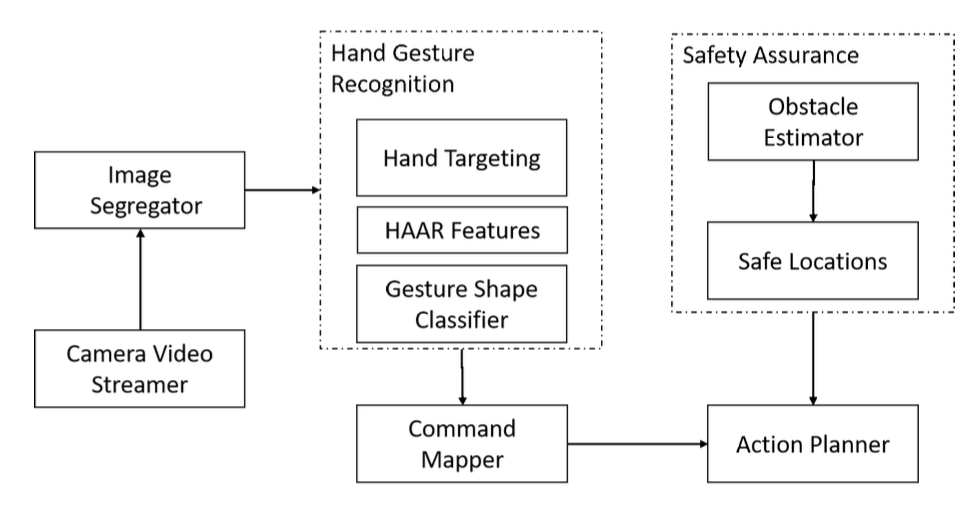
\includegraphics[width=0.8\textwidth]{Haar2.png}
    \caption{چارچوب کنترل پهپاد مبتنی بر ژست}
\end{figure}


\begin{figure}[h]
    \centering
    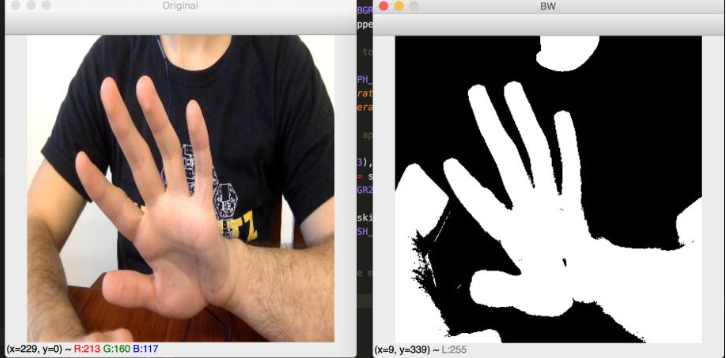
\includegraphics[width=0.5\textwidth]{Haar3.png}
    \caption{ ویژگی های \lr{Haar} برای استفاده از آستانه رنگ پوست برای تشخیص دست}
\end{figure}




\subsubsection{نتیجه بدست آمده}
این پروژه دقت بالایی در تشخیص ژست دست و کنترل پرواز پهپاد دارد. پنج حالت دست مدنظر در این پروژه قرار گرفته‌اند و دقت متوسط آن برابر با ۴۷۱.۹۷ درصد 
است که نشان‌دهنده عملکرد بسیار عالی است. اما لازم به ذکر است که این دقت در پس‌زمینه‌های بهم ریخته و همچنین در شرایط نوری مختلف 
بسیار متغیر است زیرا ویژگی \lr{Haar} به سایه و رنگ‌های درون تصویر بسیار حساس است.



\subsection{مقاله \lr{A real-time hand gesture recognition method}}
در این مقاله در زمینه پردازش تصویر و تشخیص ژست‌های دست، از روش‌های مبتنی بر مدل ظاهری \lr{Appearance Model} به عنوان یک رویکرد موثر استفاده شده‌‌است.
این روش‌ها از ویژگی‌های تصویری و حرکتی دست برای تشخیص و تعیین ژست‌های دست استفاده می‌کنند. در این مقاله، روش تشخیص ژست‌های دست به صورت زمان واقعی و 
قابل اعتماد است که از تشخیص دست، پیگیری دست\LTRfootnote{Hand tracking}، تقسیم‌بندی دست\LTRfootnote{Hand segmentation} و تشخیص ویژگی‌های مقیاس-فضا\LTRfootnote{Scale-space feature detection} برای تشخیص ژست‌های دست استفاده می‌کند.

\subsubsection{روش‌شناسی}
در مقاله از ترکیب متنوعی از روش‌ها و ویژگی‌های تصویری استفاده می‌شود. این ویژگی‌ها به ترتیب به صورت زیر عمل می‌کنند.
\begin{enumerate}
    \item استفاده از روش \lr{Adaboost} برای تشخیص دست، که یک روش معتبر برای تشخیص اشیاء در تصاویر است.
    \item پیگیری دست با استفاده از تشخیص حرکت و رنگ، که از ترکیب تکنیک‌های جریان نوری و نشانه رنگ برای پیگیری دست در تصاویر استفاده می‌شود.
    \item تقسیم‌بندی دست با استفاده از اطلاعات حرکت و رنگ برای تمایز دست از پس‌زمینه و اشیاء دیگر. 
    \item تشخیص ویژگی‌های مقیاس-فضا برای تشخیص ژست‌های دست، که برای شناسایی ساختارهای شبیه به کف دست و انگشتان استفاده می‌شود تا نوع ژست دست توسط ترکیب این ساختارها تعیین شود.
\end{enumerate}
  این روش‌ها و ویژگی‌ها با هم ترکیب شده‌اند تا یک سیستم تشخیص دست پایدار و دقیق برای استفاده در رابط کاربری تعاملی و تشخیص ژست‌های دست در زمینه‌های مختلف ارائه شود.

\begin{figure}[h]
    \centering
    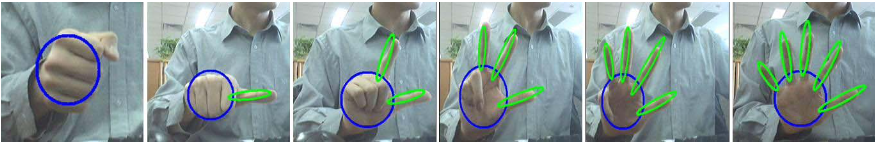
\includegraphics[width=0.8\textwidth]{hand_gesture_feature.png}
    \caption{تشخیص کف دست و انگشتان}
\end{figure}

\subsubsection{نتیجه}
اعمال این روش‌ها نتایج قابل قبولی را به همراه داشته است. دقت مدل در تشخیص ژست‌های دست به صورت میانگین 8.93 درصد بوده و از جمله نتایج مهم آزمایشات می‌توان به تشخیص 
صحیح 2436 فریم از کل 2596 فریم ضبط شده اشاره کرد. این نتایج نشان می‌دهند که روش ارائه شده در این مقاله عملکرد قابل قبولی در تشخیص ژست‌های دست دارد و 
می‌تواند به عنوان یک روش موثر برای تعاملات زمان واقعی استفاده شود.
\cite{fang2007real}


\subsection{مقاله \lr{Hand Gesture Recognition using Image Processing and Feature Extraction Techniques}}

\subsubsection{روش‌شناسی}

\subsubsection{نتیجه}
\cite{sharma2020hand}



\section{مقالات مربوط به ورودی تصویر دست به مدل}
مقالات این دسته از جمله پرژه‌هایی هستند که بیشتر از آنکه بر روی پیش پردازش کار کنند باید بر روی معماری خود شبکه تمرکز کنند. در این مقالات تمام یا بخشی از تصویر گرفته شده به صورت یک ماتریس از تصویر با پیکسل‌های متعدد به مدل داده می‌شود. تنها موردی که می‌توان در این نوع پروژه‌ها پیش رو گرفت تشخیص موقعیت دست است تا بتوان تنها قسمتی از تصویر را به ورودی شبکه داد که دست در آن وجود دارد تا در حد ممکن انداژه ورودی شبکه و دقت آن افزایش یابد. پس از آن باید توجه داشت معماری شبکه را به گونه‌ای برگزید تا مخصوص پردازش تصویر باشد و بتوان ویژگی‌های تصویر را خود استخراج کند.


\subsection{مقاله \lr{Hand Gestures For Drone Control Using Deep Learning}}
این پروژه با هدف کنترل پهپادها با استفاده از حرکات دستی و با کمک شبکه‌های عمیق یادگیری انجام شده است تا بتوان ۹ حالت مختلف دست را شناسایی و به پهپاد، دستور موردنظر کاربر را داد.


\subsubsection{روش‌شناسی}
در این تحقیق، از معماری شبکه عصبی عمیق \lr{VGG-16} برای تشخیص و تعیین حرکات دستی برای کنترل پهپادها استفاده شده است. شبکه \lr{VGG-16} یکی از معروف‌ترین و پرکاربردترین شبکه‌های عمیق در زمینه بینایی ماشین است که 
شامل 16 لایه عصبی با لایه‌های کانولوشنال و پولینگ می‌باشد. این شبکه برای استخراج ویژگی‌های مهم از تصاویر استفاده می‌شود. ورودی این شبکه تصاویری است که از دوربین متصل به دستگاه اجرایی گرفته می‌شود و سپس این 
تصاویر به شبکه وارد می‌شوند. خروجی این شبکه شامل تشخیص حرکات دستی مانند حرکات مختلف انگشتان و دست‌ها می‌شود که سپس این اطلاعات برای ارسال دستورات کنترلی به پهپاد استفاده می‌شود. این روش نه تنها امکان کنترل دقیق 
و موثر پهپادها را فراهم می‌کند بلکه ارتباط بین انسان و ماشین را نیز بهبود می‌بخشد.

\begin{figure}[h]
    \centering
    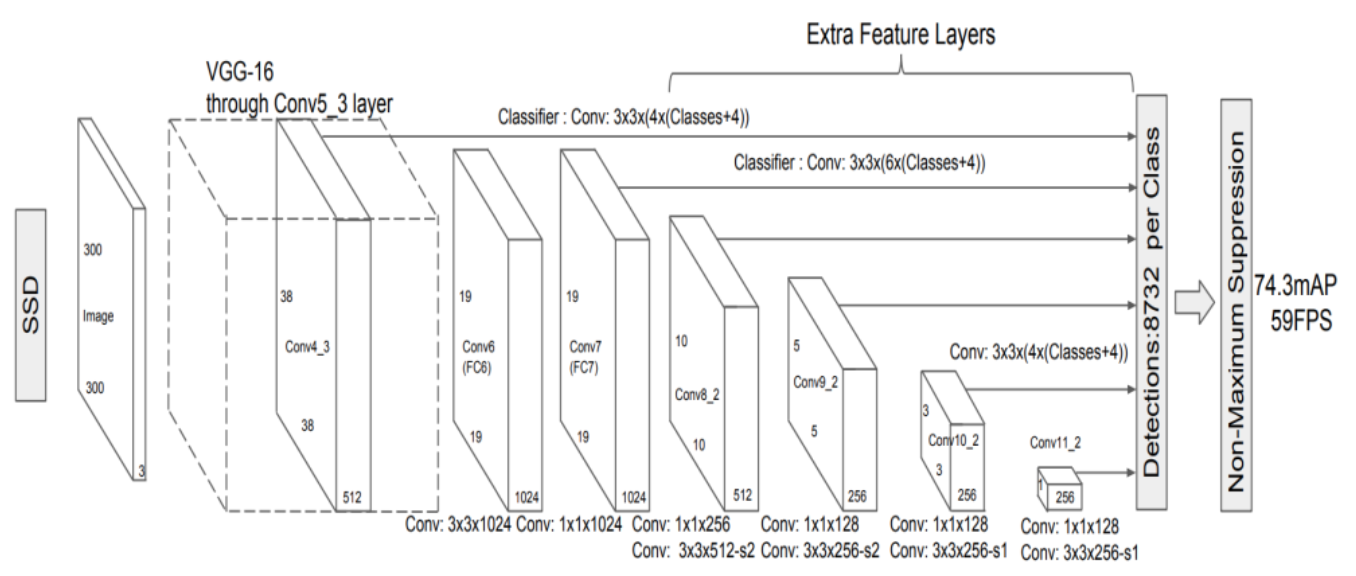
\includegraphics[width=0.8\textwidth]{VGG16.png}
    \caption{معماری \lr{VGG-16}}
\end{figure}

\subsubsection{نتیجه بدست آمده}
 در پروژه این پروژه ۹ حالت دست مدنظر قرار گرفته‌شده و دقت آن برابر ۳.۸۳ درصد است.
 که در بهترین حالت ممکن با پس‌زمینه‌ی مناسب بدست آمده و باید در نظر گرفت که دقت بالایی برای کنترل پهپاد به حساب نمی‌آید.
\cite{hadri2018hand}

\subsection{مقاله \lr{UAV-GESTURE: A Dataset for UAV Control and Gesture Recognition}}
این مقاله به منظور کنترل پهپاد یا خلبان خودکار با استفاده از حرکت دست پیاده‌سازی شده است. به عنوان مثال، حرکت دست از چپ به راست نشان‌دهنده حرکت پهپاد به راست می‌باشد. 
برای اجرای این برنامه، شبکه \lr{P-CNN} طراحی شده است تا بتواند مفهوم تصاویر را تجربه کند.

\subsubsection{روش‌شناسی}
در این مقاله، از شبکه \lr{P-CNN} \LTRfootnote{Pose-based Convolutional Neural Network} برای تشخیص حرکات دست استفاده شده است. این شبکه از اطلاعات حرکت و ظاهر را بر روی مسیرهای بخش‌های بدن انسان (مانند دست راست، 
دست چپ، بدن بالا و بدن کامل) جمع‌آوری می‌کند. این شبکه ابتدا موقعیت دست فرد را با استفاده از جعبه مرزی مشخص می‌کند و سپس تصویر دست با استفاده از فیلترهای مناسب وارد شبکه \lr{P-CNN} می‌شود تا بتواند حرکت دست را پیش‌بینی کند.
\\
در خروجی این مدل، ۱۳ نوع حرکت مختلف وجود دارد که برای پیش‌بینی مفهوم آن‌ها استفاده می‌شود. این حرکات شامل کل دست از شانه تا انگشتان و حرکات آنها می‌شود، که در این پروژه برای دستور دادن به هواپیماهای بزرگ بدون سرنشین در فرودگاه‌ها استفاده می‌شود.
\\
\lr{P-CNN} اطلاعات ظاهر و حرکت را از بخش‌های مختلف بدن استخراج می‌کند و از دو شبکه پیش‌آموزش داده شده برای محاسبه ویژگی‌های \lr{CNN} استفاده می‌کند. برای بخش‌های ظاهر، از شبکه \lr{VGG-f} استفاده می‌شود، در حالی که برای 
بخش‌های حرکتی از شبکه حرکتی از پیاده‌سازی \lr{Action Tube} استفاده می‌شود. ویژگی‌های استاتیک و پویا به طور جداگانه در طول زمان جمع‌آوری می‌شوند تا ویژگی‌های ویدیوی استاتیک و پویا به دست آید.
\\
در نهایت، از روش‌های تجمیع مینیمم و ماکسیمم برای هر بعد از توصیف‌گر بر روی تمام ویدیوها استفاده می‌شود. این روش‌ها برای تشخیص حرکات با دقت بالا استفاده می‌شوند.



\subsubsection{نتیجه}
دارد، اما نیازمندی‌های پیچیده‌ای برای پیاده‌سازی واقعی دارد که از جمله موانعی است که باید در نظر گرفته شود.
در نتیجه، این مقاله یک روش برای کنترل پهپاد با استفاده از حرکت دست پیاده‌سازی کرده است و از شبکه \lr{P-CNN }
برای تشخیص حرکات دست استفاده کرده است. نتایج نشان داده‌اند که این روش با دقت ۹.۹۱ درصد، قابلیت اجرا در پروژه‌های واقعی را دارد، اما نیازمندی‌های پیچیده‌ای برای پیاده‌سازی واقعی دارد که از جمله موانعی است که باید در نظر گرفته شود.
\cite{perera2018uav}




\section{مقالات مربوط به نقاط کلیدی دست}
در این چنین مقالات ورودی شبکه بینایی ماشین برای تشخیص ژست، مختصات نقاط کلیدی دست هستند، که به نوعی یک ویژگی تصویر نیز تلقی می‌شوند. بدین صورت که در ابتدای کار دست کاربرد شناسایی شده و سپس نقاط کلیدی آن استخراج می‌شوند تا بتوان حجم داده ورودی به مدل را تا حد امکان ساده‌تر و در عین حال مفیدتر کرد.

\subsection{مقاله \lr{Hand Gesture Recognition system for Real-Time Application}}
% این مقاله به بررسی سیستم تشخیص حرکات دست برای کاربردهای زمان واقعی می‌پردازد. در این سیستم، از الگوریتم SIFT برای استخراج ویژگی‌ها از تصاویر 
% حرکتی استفاده شده و سپس از مدل Bag of Feature و رده‌بند SVM برای تشخیص دقیق حرکات دست و دستیابی به عملکرد زمان واقعی استفاده شده است.

% \subsubsection{روش‌شناسی}
% در این مقاله، از الگوریتم SIFT برای استخراج نقاط کلیدی دست از تصویر استفاده شده است. این نقاط برای تشخیص دقیق حرکات دست و دستیابی به عملکرد زمان واقعی مورد استفاده قرار گرفته‌اند. 
% برای پیدا کردن نقاط کلیدی دست از الگوریتم SIFT استفاده می‌شود تا بتوان ویژگی‌های برجسته و تمایزدهنده  تصاویر را استخراج کرد. دلیل استفاده از این 
% الگوریتم به این دلیل است که نقاط دست از مقیاس، جهت و بخشی از تغییرات نوری مستقل هستند و می‌توان از آنها برای تطبیق قابل اعتماد بین دیدگاه‌های مختلف یک شیء یا تصویر استفاده کرد. 

% \subsubsection{نتیجه}
% در این پروژه که برای استخراج نقاط کلیدی دست از الگوریتم SIFT استفاده شده، عملکرد مدل برابر دقت 90.8٪ در تشخیص حرکات دست است.
\cite{murugeswari2014hand}


\subsection{مقاله \lr{An improved hand gesture recognition system using keypoints and hand bounding boxes}}
این مقاله یک سیستم بهبود یافته تشخیص حرکات دست با استفاده از نقاط کلیدی و جعبه‌های محدود کننده دست را معرفی می‌کند تا بتوان نقاط کلیدی دست را پیدا کرد.


\subsubsection{روش‌شناسی}
این پروژه از دو لوله موازی به نام‌های "\lr{MobileNetV2 + FC}" و "\lr{CNN + FC}" تشکیل شده‌است که تصاویر جعبه 
محدود کننده دست و ویژگی‌های استخراج شده از نقاط کلیدی را ترکیب می‌کند و از این طریق ژست دست را پیش‌بینی می‌کند. 
\\
در مدل \lr{MobileNetV2 + FC}، از یک معماری سبک به نام \lr{MobileNetV2} برای استخراج ویژگی‌ها از تصاویر جعبه 
محدود کننده دست استفاده می‌شود. سپس این ویژگی‌ها به یک شبکه عصبی کاملاً متصل (\lr{FC}) داده می‌شوند تا حرکات دست تشخیص داده شوند.
\\
در مدل \lr{CNN + FC} ، در ابتدا نقاط کلیدی دست  که اطلاعات مهمی درباره حرکات دست را شامل می‌شوند پیدا کرده و به یک شبکه عصبی کاملاً متصل (\lr{FC}) وارد می‌شوند تا حرکات دست
تشخیص داده شوند. این مدل از لایه‌های کانولوشنی برای کاهش تعداد پارامترها استفاده می‌کند و سپس از لایه‌های کاملاً متصل برای تشخیص حرکات دست استفاده می‌کند.

\begin{figure}[h]
    \centering
    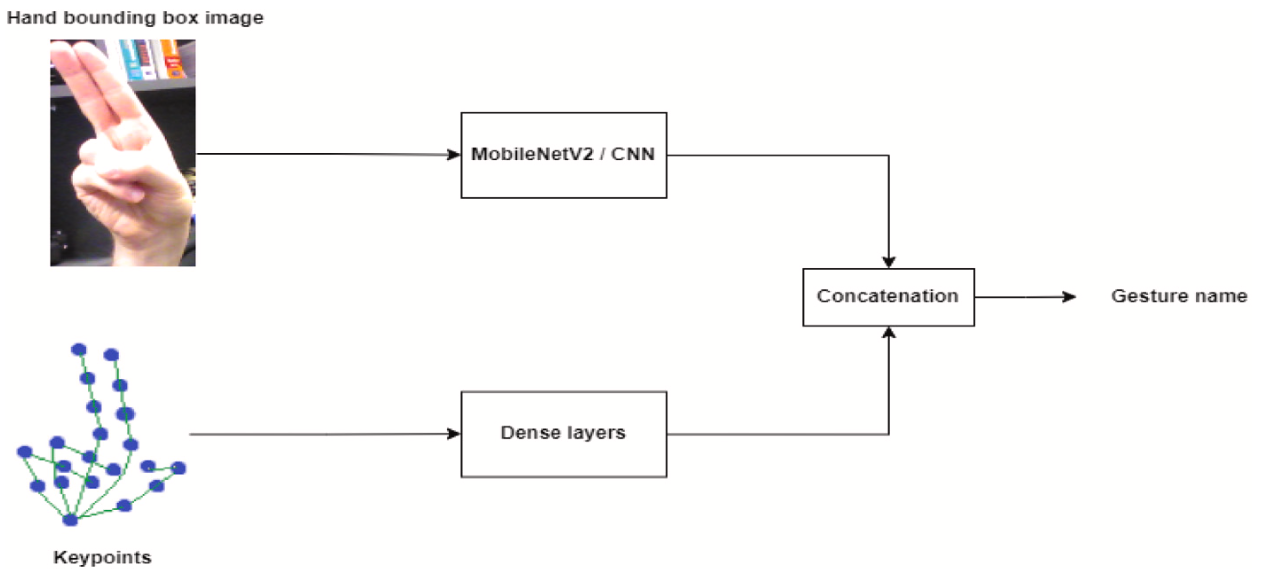
\includegraphics[width=0.8\textwidth]{keypoints_boundingBox.png}
    \caption{معماری ساختار شبکه‌های عصبی دو خط لوله}
\end{figure}


\subsubsection{نتیجه}
در صورتی که دو مدل خروجی‌های متفاوتی را پیش‌بینی کنند، از روش‌های ترکیبی مانند ترکیب احتمالاتی یا استفاده از مدل‌های متفاوت برای شرایط ورودی مختلف استفاده می‌شود تا بهترین تصمیم برای تشخیص ژست دست گرفته شود.



\cite{dang2022improved}


\subsection{مقاله \lr{Visual gesture recognition based on hand key points}}

\subsubsection{روش‌شناسی}

\subsubsection{نتیجه}
\cite{chen2021visual}.


\subsection{مقاله \lr{MediaPipe Hands: On-device Real-time Hand Tracking}}
در این مقاله‌ها از کتابخانه \lr{MediaPipe} استفاده‌ شده‌است تا بتوان ۲۱ نقطه عطف دست را پیدا کرده و در پروژه‌های گوناگون از جمله پیدا کردن ژست دست و افکت‌های \lr{AR} استفاده کند. ما در پروژه خود از این کتابخانه استفاده می‌کنیم تا بتوانیم مدلی سبک و ساده پیاده کنیم.

\subsubsection{روش‌شناسی}
 در این مقاله به یررسی این کتابخانه پرداخته‌شده و ما از آن استفاده می‌کنیم تا بتوانیم مدلی برای پیش‌بینی ژست دست استفاده کنیم.
برای پیاده‌سازی این پروژه از دو شبکه کانولوشن استفاده شده است. شبکه اول که برای پیدا کردن کف دست در تصویر استفاده می‌شود و شبکه دوم که به عنوان ورودی موقعیت عکس دست پیدا شده را دریافت و مختصات ۲۱ تقطه عطف را موقعیت‌یابی می‌کند.

\subsubsection{نتیجه}
مدل‌های طراحی شده در این مقالات برای تشخیص نقاط عطف دست از دقت ۷.۹۵ درصد برخوردار هستند که دقت بسیار بالایی محاسبه می‌شود. همچنین این مدل به نور و تصویر پس‌زمینه وابسته نیست و دقت متوسط آن در زمینه‌های مختلف اندازه‌گیری شده لذا مدل را کاربردی‌ و مورد پسندتر می‌کند
\cite{zhang2020mediapipe} 







\section{مقالات مربوط به اجرای مدل‌های بینایی کامپیوتر روی پهپاد}
\subsection{مقاله \lr{Modeling relation among implementing AI-based drones and sustainable construction project success}}

\subsubsection{روش‌شناسی}

\subsubsection{نتیجه}

\section{جمع‌بندی}
\cite{waqar2023modeling}

\subsection{مقاله \lr{}}

\subsubsection{روش‌شناسی}

\subsubsection{نتیجه}
\cite{}


در تمام مقالات بررسی شده، پروژه‌ها به گونه‌ای پیاده‌سازی شده‌اند تا حرکات را به طوری کلاس‌بندی کنند که در خروجی حتما یکی از ژست‌های درنظر گرفته‌شده انتخاب شود. لذا زمانی که دست در حالتی غیر از آنها قرار دارد، مدل طراحی شده حتما یکی از ژست‌هایی را که به آن شبیه‌تر است را انتخاب می‌کند که این امر می‌تواند برای پیاده‌سازی روی پهپاد واقعی مشکل‌زا باشد و حتی هزینه مالی به ارمفان آورد.

استخراج ویژگی‌های تصویر و یا ورودی خود تصویر به مدل می‌تواند بهینه عمل نکند